
\documentclass{article}
\usepackage{paper_style} 
\usepackage[a4paper, left=30mm, top=20mm, right=15mm, bottom=20mm, nohead, includefoot,footskip=35pt]{geometry}


\usepackage{chemfig}

\begin{document}
\tableofcontents

\pagebreak
\section{Интеграл  NURBS кривой}

Рассматривается задача нахождения аналитического интеграла для NURBS $p$-ой степен кривой, заданной в виде \cite{nurbs_book}:

\begin{equation} \label{NURBS_def}
    C(t)=\frac{\sum_{i=0}^{n} N_{i, p}(t) w_{i} P_{i}}{\sum_{i=0}^{n} N_{i, p}(t) w_{i}}, \quad a \leq t \leq b,
\end{equation}
где $\left\{P_{i}\right\}$ множество контрольных точек; $\left\{w_{i}\right\}$ вектор весов, причем $w_i>0$;\\
$\left\{N_{i, p}(t)\right\}$ -- базисные В-сплайн функции $p$-ой степени, определенных на векторе узлов:

\[
    U=\{\underbrace{a, \ldots, a}_{p+1}, t_{p+1}, \ldots, t_{m-p-1}, \underbrace{b, \ldots, b}_{p+1}\}.
\]

Пусть кривая C(t) на каждом $k$-м сегменте определена, как 

\begin{equation} \label{NURBS}
    C_k(t)=\left( \frac{P_x(t)}{Q(t)}, \frac{P_y(t)}{Q(t)} \right).
\end{equation}

Интеграл для каждого $k$-го сегмента NURBS кривой определяется следующим образом:

\begin{equation} \label{NURBS_integral_segment}
	I_k = \int_{t_{k}}^{t_{k+1}} y(t) x'(t) d t = 
	\int_{t_{k}}^{t_{k+1}} \frac{P_{y}(t)\left(P_{x}^{\prime}(t) Q(t)-Q^{\prime}(t) P_{x}(t)\right)}{Q^{3}(t)} d t. 
\end{equation}

Разобьём интеграл $I_k$ на два интеграла $I_1$ и $ I_2$:

\begin{equation} \label{I_1_before}
	I_1 =  \int_{t_{k}}^{t_{k+1}} \frac{P_{y}(t) P_{x}^{\prime}(t) Q(t)}{Q^{3}(t)}dt =  \int_{t_{k}}^{t_{k+1}} \frac{P_{y}(t) P_{x}^{\prime}(t)}{Q^{2}(t)}dt,
\end{equation}

\begin{equation} 
	I_2 =  - \int_{t_{k}}^{t_{k+1}} \frac{P_{y}(t) Q^{\prime}(t) P_{x}}{Q^{3}(t)}dt.
\end{equation}

Далее упростим выражение $I_1$ (\ref{I_1_before}): 

Имеем $deg P_x(t) = deg P_y(t) = p$, $ degQ(t)=m$, $ m\le p$.
Поделим многочлен $P_y(t)$ c остатком $ \frac{P_y(t)}{Q} = P_1(t) + \frac{R_1(t)}{Q(t)} $, \ где $ degR_1(t) < degQ(t)$.
Аналогично поделим $ \frac{P'_x(t)}{Q} = P_2(t) + \frac{R_2(t)}{Q}$, где $ degR_2(t) < degQ(t)$.

Интеграл $I_1$ принимает вид:
\begin{equation} \label{I_1}
	I_1 = \int_{t_{k}}^{t_{k+1}} P_1(t)P_2(t) dt + 
	 \int_{t_{k}}^{t_{k+1}} \frac{P_1(t) R_2(t) + P_2(t) R_1(t)}{Q(t)} dt + 
	 \int_{t_{k}}^{t_{k+1}} \frac{R_1(t)R_2(t)}{Q^2(t)} dt.
\end{equation}

Для разложения $G(t) = \frac{P_1 R_2 + P_2 R_1}{Q}$ на простейшие дроби применим метод Хевисайда.
Для начала поделим многочлены и получим $ G(t) = P_3 + \frac{R_3}{Q}$, где $ degR_3 < degQ = m$.

Для рациональной функции $ \frac{R_3(t)}{Q(t)} = \frac{R_3(t)}{(t-a_1) \cdot \ldots \cdot (t-a_m)}$ требуется найти коэффициенты $B_k$, участвующие в разложении: 
$ G(t) = \sum_{k=1}^{m} \frac{B_{k}}{\left(t-a_{k}\right)}$.
Метод позволяет найти коэффициенты $B_k \in  \mathbb{C}$ напрямую:
\begin{equation} \label{Heaviside}
B_{k}=\left.\frac{P(t)(t-a_k)}{Q(t)}\right|_{t=a_k} = \frac{P(a_k)}{\prod_{j \ne k}{(a_k - a_j)}}.
\end{equation}


Для нахождения третьего слагаемое в выражении (\ref{I_1}) разложим по отдельности $ \frac{R_1(t)}{Q(t)}$ 
и $\frac{R_2(t)}{Q(t)}$. Получим : 

\begin{equation} \label{two_sum}
	\sum_{k=1}^m \frac{A_{k}}{\left(t-a_{k}\right)} \cdot 
	\sum_{k=1}^m \frac{B_{k}}{\left(t-a_{k}\right)} = 
	\sum_{k=1}^m \frac{A_{k} B_{k}}{\left(t-a_{k}\right)^2} +
	\sum_{k=1}^m  \sum_{j=k+1}^m \frac{A_{k} B_{j} + A_{j} B_{k}} {\left(t-a_{j}\right)\left(t-a_{k}\right) }.
\end{equation}

Интеграл от выражений типа $ \frac{C}{(t-a_j)(t-a_k)}$, где $ j \ne k,  C \in  \mathbb{C}$, будем находить повторным разложением методом Хевисайда. \\

Для нахождения производной многочлена Q, представленного в виде
$ Q(t) = (t-a_1) \cdot \ldots \cdot (t-a_m)$, \ где $a_i \in  \mathbb{C}$,
используем свойства производной произведения:
\begin{equation}
	Q'(t)=Q(t) \cdot \left( \frac{1}{t - a_1} + \ldots + \frac{1}{t - a_m} \right).
\end{equation}

Тогда интеграл $I_2$ будет выглядеть:

\begin{equation} \label{I_2}
	I_2 =  - \sum_{j=1}^{m} I_{2j} ,\  \text{где} \ I_{2j} = \int_{t_{k}}^{t_{k+1}} \frac{P_y(t) P_x(t)}{Q^2(t) (t - a_j)}.
\end{equation}

Как можно заметить, максимальная степень знаменателя в подынтегральных выражениях $I_1$ и $I_2$ уменьшилась.

Упростим $j$-ый член суммы в интеграле $I_2$. Аналогично $I_1$ получим:

\begin{equation} \label{div1}
	\frac{P_y(t)}{Q(t)} = P_1 + \frac{R_1(t)}{Q(t)}, \ \text{где} \ \ degR_1 < degQ=m,
\end{equation}

\begin{equation} \label{div2}
	\frac{P_x(t)}{Q(t)} = P_2 + \frac{R_2(t)}{Q(t)}, \ \text{где} \ \ degR_2 < degQ=m.
\end{equation}

Подставив (\ref{div1}) и (\ref{div2}) в (\ref{I_2}), получим:
\begin{equation} \label{I_2j}
	I_2j = \int_{t_{k}}^{t_{k+1}} \frac{P_1P_2}{t-a_j} dt + 
		  \int_{t_{k}}^{t_{k+1}} \frac{P_1 R_2 + P_2 R_1}{Q(t)(t-a_j)} dt + 
		  \int_{t_{k}}^{t_{k+1}} \frac{R_1R_2}{Q^2(t)(t-a_j)} dt.
\end{equation}
\begin{equation} \label{div3}
	\frac{P_1(t)P_2(t)}{t-a_j} = P_3(t) + \frac{R_3}{t-a_j}, \ \text{где} \ \ R_3 \in  \mathbb{C}.
\end{equation}

\begin{equation} \label{div4}
	\frac{P_1(t) R_2(t) + P_2(t) R_1(t)}{t-a_j} = P_4(t) + \frac{R_4}{t-a_j}, \ \text{где} \ \ R_4 \in  \mathbb{C}.
\end{equation}

Итого получаем:

\begin{multline}
	I_2j = \int_{t_{k}}^{t_{k+1}} \left[P_3(t) + P_4(t)\right] dt +
	\int_{t_{k}}^{t_{k+1}} \frac{R_3}{t-a_j} dt  \ + \\
	+ \int_{t_{k}}^{t_{k+1}} \frac{R_4}{Q(t)} dt + 
	\int_{t_{k}}^{t_{k+1}} \frac{R_1(t)R_2(t)}{Q^2(t)(t-a_j)} dt.
\end{multline}

Первые два слагаемые находятся непосредственно. Оставшиеся вычисляются аналогично методам (\ref{Heaviside}) и (\ref{two_sum}), использованных при нахождении $I_1$ .

\section{Асимптотическая оценка алгоритма}

Пусть $deg P_x(t) = deg P_y(t) = degQ(t) = p$
Тогда при делении с остатком:



\section{Оценка алгоритма}

Сравним полученный алгоритм с методом, использующим разложения дроби на простейшие с помощью метода неопределенных коэффициентов.




\section{Результаты}

\begin{figure}[H]
    \centering
    \begin{subfigure}[b]{0.49\textwidth}
        \centering
        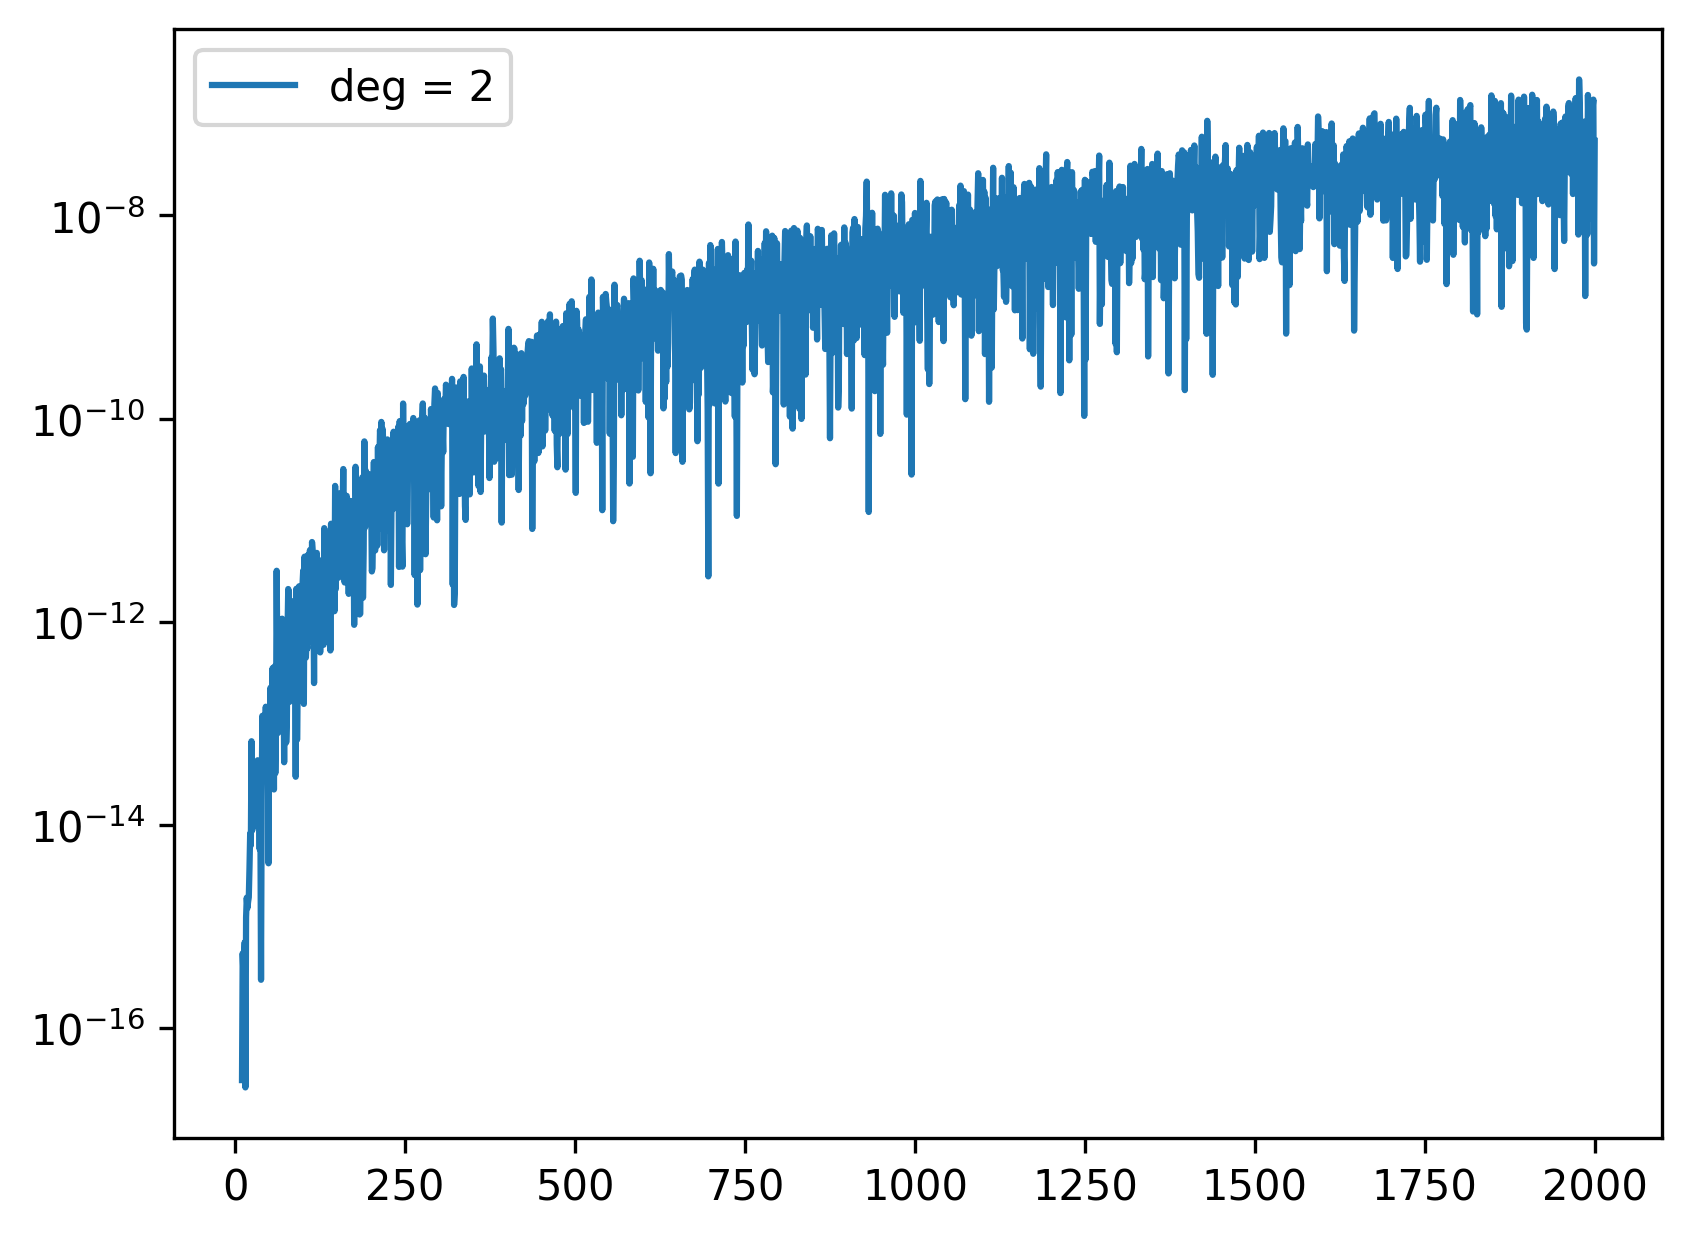
\includegraphics[width=\textwidth]{src/errors_2_2000.png}
        \caption{Сравнение аналитического и численного интеграла NURBS  кривой}\label{fig:plot3}
    \end{subfigure}
    \hfill
    \begin{subfigure}[b]{0.49\textwidth}
        \centering
        \includegraphics[width=\textwidth]{src/errors_234_500.png}
        \caption{Сравнение аналитического и численного интеграла NURBS  кривой}\label{fig:errors3}
    \end{subfigure}
       \caption{Сравнение численной и аналитической $B$-сплайн кривой $p=3$, $n=20$ контрольных точек}
       \label{fig:compare_bspline_3}
\end{figure}

Сравним полученный алгоритм для нахождения интеграла NURBS кривых 

Сравнивать будем с численным интегралом
//код


Замечание. Данный алгоритм 
\pagebreak
\section{Параметризация [0, 1]}

Для каждого сегмента сделаем замену $t  = (t_{k+1}-t_{k}) \tau  + t_k$, где 
$ \tau \in [0, 1]$.
Тогда модифицированный алгоритм де-Бура будет выглядит следующим образом:

\begin{lstlisting}[language=C++,frame=single,caption=Модифицированный алгоритм де Бура для построения полиномов NURBS кривой с параметризацией \text{[0, 1]}.,label=code1]
template<typename T>
Rational<T> de_boor_nurbs2(int k1, int k2, std::vector<T>& knots,
                          std::vector<T>& weights,
                          std::vector<Point<T>>& points, int p) {
    size_t dim = points[0].dim;
    std::vector<Point<Poly<T>>> d((size_t)p+1, Point<Poly<T>>(dim));
    std::vector<Poly<T>> d_den((size_t)p+1);
    for (int i = 0; i < p+1; ++i){
        d_den[i][0] = weights[i + k1 - p];
        for (int j = 0; j < dim; ++j)
            d[i][j][0] = points[i + k1 - p][j] * weights[i + k1 - p];
    }
    T B,D, den;
    Poly<T> poly_up({knots[k2] - knots[k1], knots[k1]});
    Poly<T> poly_up_neg({knots[k1] - knots[k2], - knots[k1]});

    for (int r = 1; r < p+1; ++r) 
        for (int j=p ; j > r-1; --j) {
            den = knots[j+1+k1-r] - knots[j+k1-p];
            B = - knots[j+k1-p];
            D = knots[j+1+k1-r];
            Poly<T> temp1_den = d_den[j] * poly_up + B * d_den[j];
            Poly<T> temp2_den = d_den[j-1] * poly_up_neg + D * d_den[j-1];
            d_den[j] = (temp1_den + temp2_den) / den;
            for (size_t i = 0; i < dim; ++i){
                Poly<T> temp1 = d[j][i] * poly_up + B * d[j][i] ;
                Poly<T> temp2 = d[j-1][i] * poly_up_neg + D * d[j-1][i];
                d[j][i] = (temp1 + temp2) / den;
            }
        }
    return {d[p], d_den[p]};
}
\end{lstlisting} 


Благодаря данной параметризации, снижается максимальный модуль коэффициентов многочленов числителя и знаменателя для каждого сегмента снижается.

\begin{figure}[H] 
    \centering
        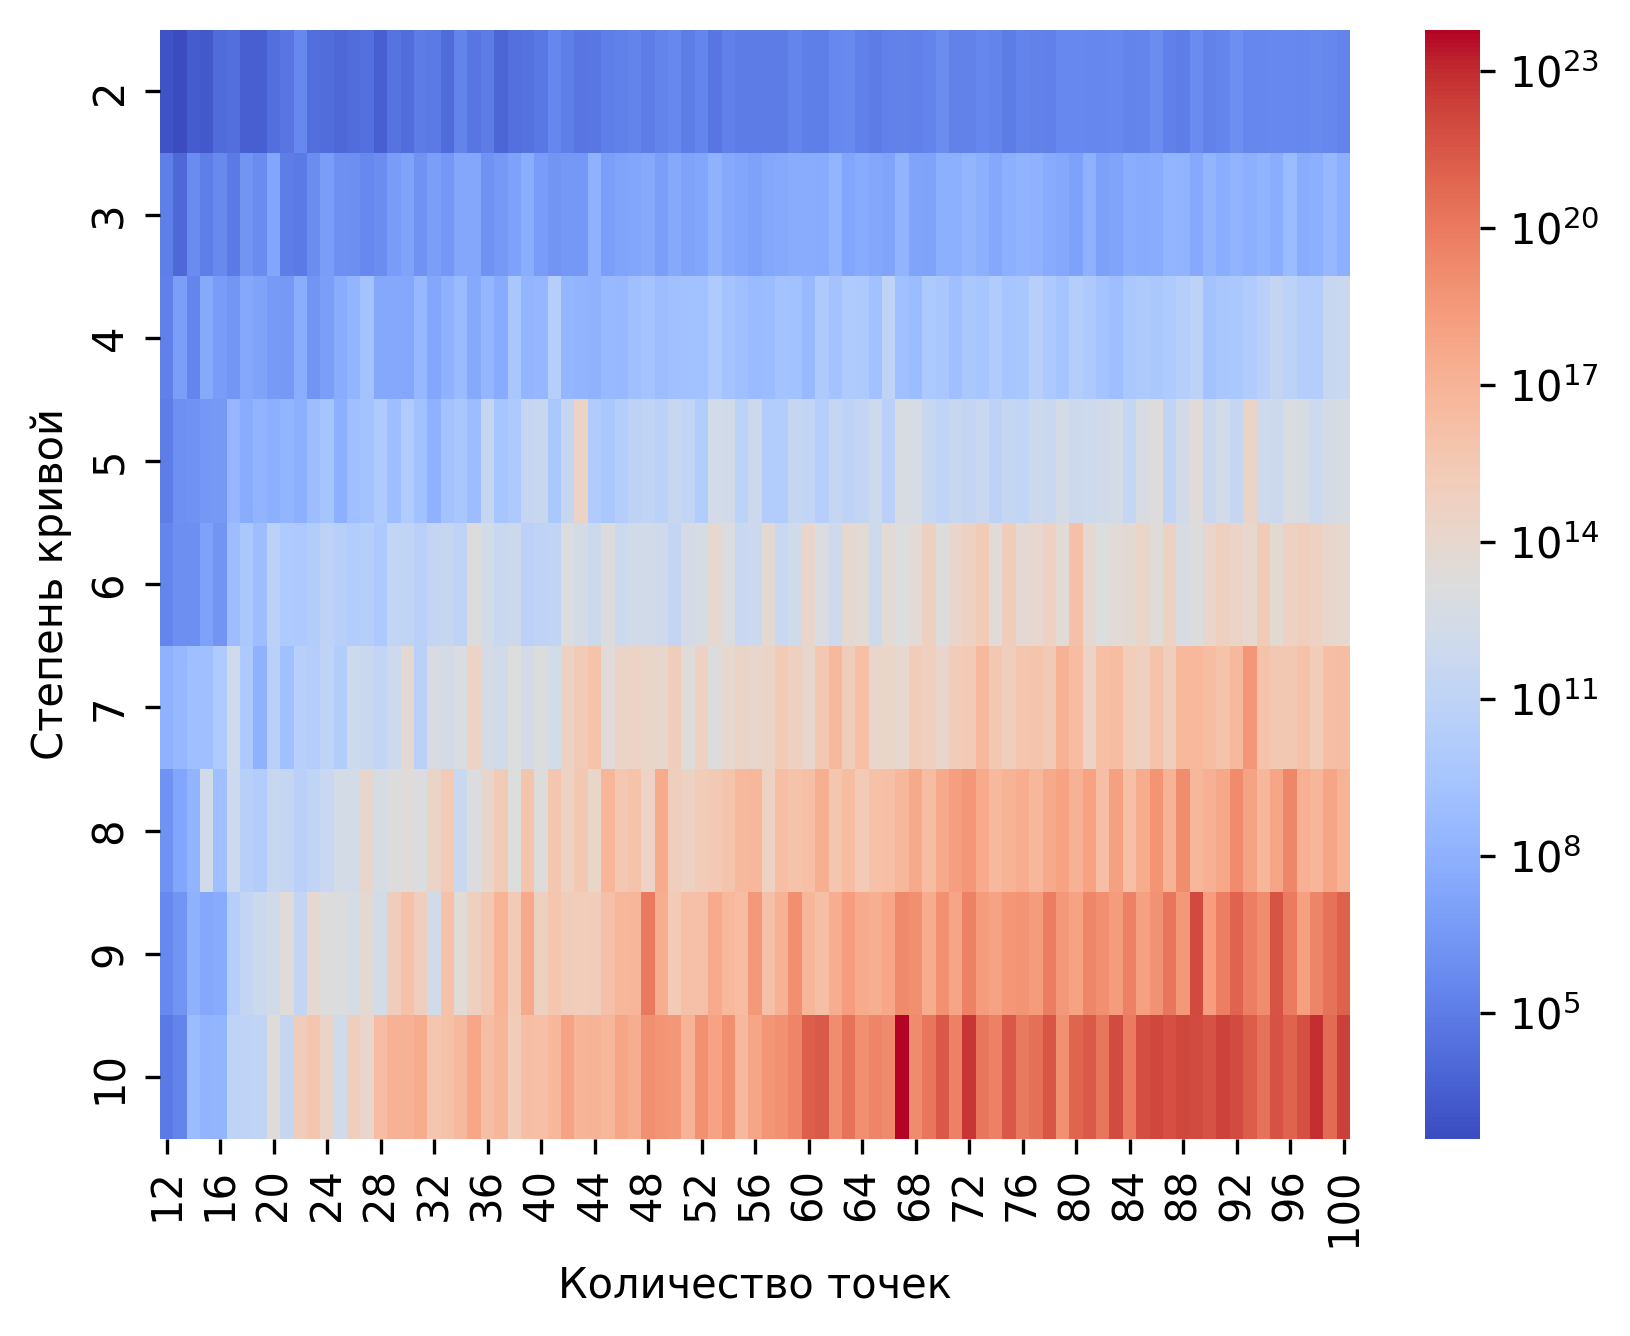
\includegraphics[width=0.6\textwidth]{src/max_coef_1.png}
        \caption {Максимальный коэффициент при стандартной параметризации}
        \label{fig:max_coef_1}
\end{figure}


\begin{figure}[H] 
    \centering
        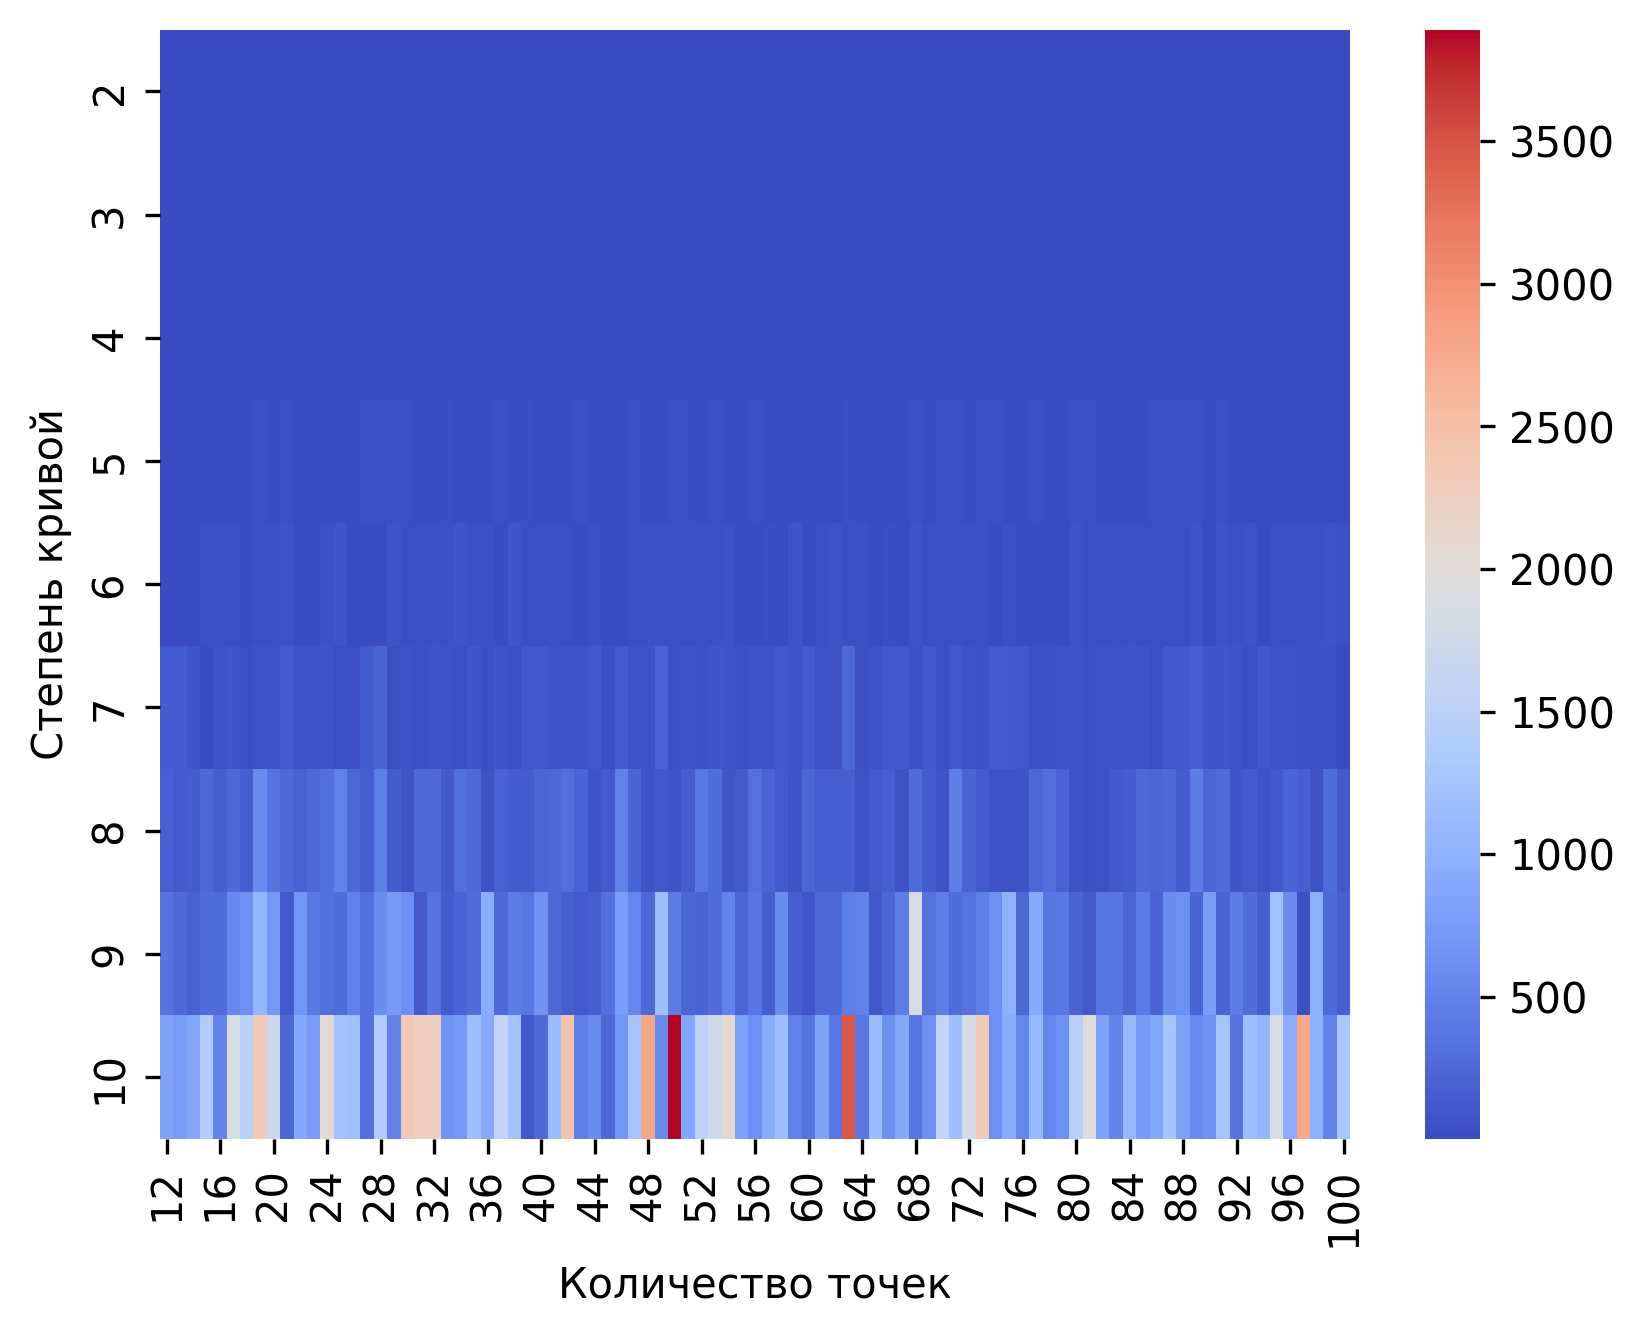
\includegraphics[width=0.6\textwidth]{src/max_coef_2.png}
        \caption {Максимальный коэффициент при параметризации [0, 1]}
        \label{fig:max_coef_2}
\end{figure}



\pagebreak
\section{Выводы}

    
\pagebreak
\begin{thebibliography}{1}
\bibitem{nurbs_book} Les Piegl, Wayne Tiller, The NURBS book/ Springer Science,  1995 – 641 с.
\end{thebibliography}

\end{document}
